\documentclass{article}
\usepackage{fullpage}
\usepackage{amssymb}
\usepackage{listings}
\usepackage{color}
\usepackage{xcolor}
\usepackage{enumerate}
\usepackage{enumitem}
\usepackage{hyperref}
\usepackage{tikz}
\usepackage[utf8]{inputenc} % åäö
\usepackage{verbatim}




% hrefs
\hypersetup{
  colorlinks=true,
  urlcolor=cyan
}




\begin{document}

  \title{ Laboration | HTML }
  \author{ IS-A | Uppsala Universitet }
  \date{ HT14 }
  \maketitle

  \lstset{language=XML}







\section*{Introduktion}
I denna labb så kommer vi att bekanta oss med \href{http://en.wikipedia.org/wiki/HTML}{HTML} och \href{http://en.wikipedia.org/wiki/Cascading_Style_Sheets}{CSS}.


\section{Mappstruktur}
Vi skulle föreslå att ni använder följande mapp/filstruktur när nu ger er in i uppgiften. Detta är inget krav, men rekommenderat.



\begin{figure}[h]
  \centering
  
  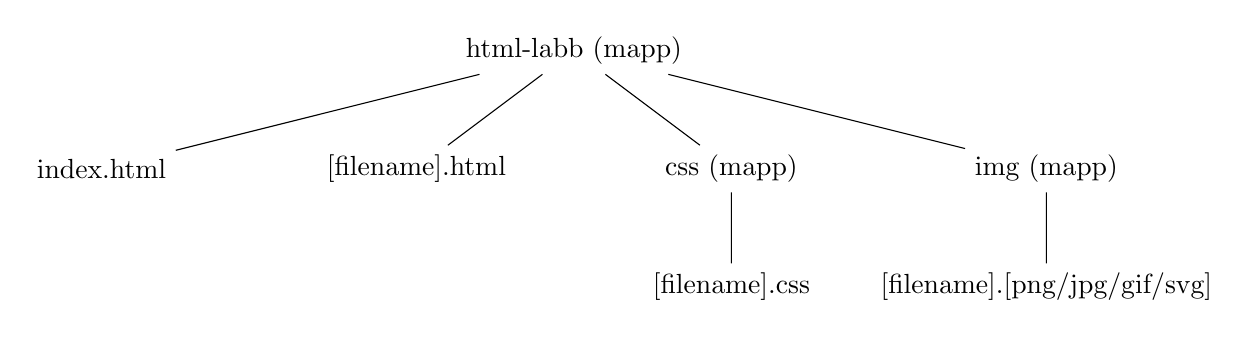
\begin{tikzpicture}[
    tlabel/.style={pos=1,right=2pt,font=\footnotesize\color{red!70!black}},
    sibling distance=4cm,
  ]

  \node {html-labb (mapp)}
  child {node {index.html}}
  child {node {[filename].html}}
  child {node {css (mapp)}
    child {node {[filename].css}}
  }
  child {node {img (mapp)}
    child {node {[filename].[png/jpg/gif/svg]}}
  }
  ;
  \end{tikzpicture}

  \caption{\emph{Förslag på mappstruktur.}}
\end{figure}





\section{Instuderingsmaterial}
För att kunna genomföra den här labben så föreslår vi att ni tar er igenom kapitel 1--3, i onlineresursen \href{http://htmlhunden.se/dist/toc.html}{HTMLHunden}. Notera att det även finns en 24 minuter lång film som pragmatiskt går igenom de mest grundläggande koncepten och begreppen -- och således fungerar som en \href{http://htmlhunden.se/dist/02-00-html-intro.html}{snabbintroduktion till webbutveckling}.





\section{Uppgiften}
Längre ned i dokumentet får du ett kodembryo som du bör utgå ifrån. Denna fil motsvarar alltså \texttt{index.html}. Koden är skriven av en slarvig programmerare och det är din uppgift att ``städa upp'' och sedan arbeta vidare med koden. Minimumkrav hittar du under rubriken ``Krav''. Huruvida du sedan vill konvertera webbsidan till ett hem för ett fiktivt företag, din egen portfolio eller bilder på katter i hattar är helt upp till dig. 



\pagebreak
\section{Krav}
\begin{enumerate}
\item Sidan måste innehålla minst en bild.
\item Sidan måste innehålla minst en extern länk.
\item Sidan måste innehålla minst en intern länk.
\item Sidan måste innehålla minst en lista \texttt{<ul>} eller \texttt{<ol>}.
\item Sidan måste innehålla minst två \texttt{html}-sidor som använder samma \texttt{css}-fil.
\item Sidan måste kunna visa bokstäverna ÅÄÖ korrekt.
\item Sidan får \textbf{inte} innehålla ``inline css''.
\item Alla ID:n måste vara unika inom en och samma \texttt{html}-sida.
\item Sidan får \textbf{inte} innehålla \texttt{<br>} eller dylik ``visuell markup'' (förutom undatag såsom \texttt{<b>} och \texttt{<i>} -- \href{http://html5doctor.com/i-b-em-strong-element/}{läs mer}).
\item Alla \texttt{html}-filer måste innehålla en ``doctype declaration'' för HTML5.
\item All kod måste vara korrekt indenterad.
\item All kod måste vara korrekt nästlad (i.e. \texttt{<div><b></div></b>}) är \textbf{inte} ok.
\item Sidan behöver göras om så att den har ett syfte -- är det en blogg? Ett fotoalbum? En sida om dig etc.
\end{enumerate}

\paragraph{Några av ovan krav}
 syftar till att hjälpa dig eliminera ``bad practice'' ifrån kodembryot. Fundera över vilka dessa är. Diskutera gärna med en labbhandledare eller kamrat.



\pagebreak
\section{Embryo}
Utgå ifrån följande kod när du börjar skapa din labblösning. Notera att nedan kod på flera sätt är ett exempel på ``bad practice''. Följ instruktionerna under rubriken ``Krav'' för att eliminiera dessa svagheter.
\verbatiminput{bad.html}






\end{document}